% Master File:lectures.tex

\lesson{Probability}
\vspace{-1cm}
\begin{center}
  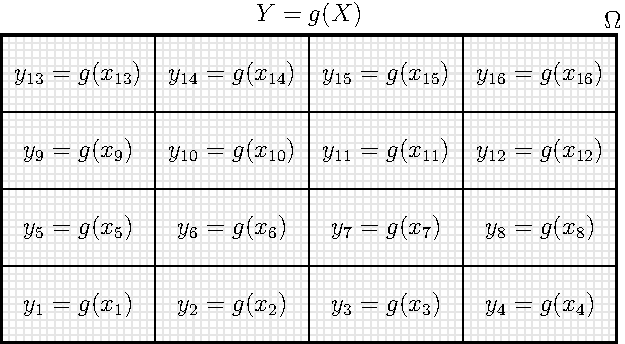
\includegraphics[height=10cm]{funcRV-1}
\end{center}
\keywords{Probability, Random Variables, Expectations}
%%%%%%%%%%%%%%%%%%%%%%% Next Slide %%%%%%%%%%%%%%%%%%%%%%%
\renewcommand{\Outline}{%
\begin{slide}
\section[1]{Outline}

\begin{minipage}{10cm}\raggedright
  \begin{enumerate}\squeeze
    \outlineitem{Random Variables}{randomv}
    \outlineitem{Expectations}{expectations}
    \outlineitem{Calculus of Probabilities}{calculus}
  \end{enumerate}
\end{minipage}\hfill
\begin{minipage}{8cm}
  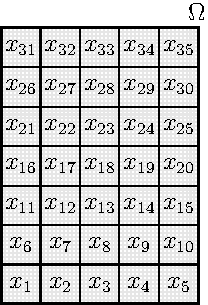
\includegraphics[width=8cm]{randomVariable}
\end{minipage}
\end{slide}
\addtocounter{outlineitem}{1}
}

\setcounter{outlineitem}{1}
\Outline % Random Variables
\toptarget{firstoutline}
%%%%%%%%%%%%%%%%%%%%%%% Next Slide %%%%%%%%%%%%%%%%%%%%%%%

\begin{slide}
\section{Modelling Uncertainty}

\begin{PauseHighLight}
  \begin{rightImage}{Omega}
    \begin{itemize}
    \item To model a world with uncertainty we consider some set of
      \emph{elementary events} or \emph{outcomes} $\Omega$\pause
    \item For the outcome of rolling a dice $\Omega=\{1,2,3,4,5,6\}$\pause
    \item The elementary events are \emph{mutually exclusive}
      $\omega_i\cap\omega_j=\emptyset$ and \emph{exhaustive} $\bigcup_i \omega_i=
      \Omega$ \pause
    \item We consider \emph{events} $\mathcal{E}=
      \bigcup\limits_{i\in\mathcal{I}}\omega_i$\pause
    \item E.g. For a dice throw $\mathcal{E} = \{2,4,6\}$\pause
    \end{itemize}
  \end{rightImage}
\end{PauseHighLight}

\end{slide}

%%%%%%%%%%%%%%%%%%%%%%% Next Slide %%%%%%%%%%%%%%%%%%%%%%%

\begin{slide}
\section[-2]{Probabilities}
  
\begin{PauseHighLight}
  \begin{itemize}
  \item We attribute a \emph{probability}, $\Prob{\mathcal{E}}$, to an event,
    $\mathcal{E}$, with the requirements
    \begin{itemize}
    \item $0\leq \Prob{\mathcal{E}} \leq 1$\pause
    \item $\Prob{\mathcal{E}} + \Prob{\neg\mathcal{E}} = 1$ where
      $\neg\mathcal{E} = \Omega \setminus \mathcal{E}$\pause
    \end{itemize}
  \item In some cases we can interpret $\Prob{\mathcal{E}}$ as the
    expected frequency of occurrence of a repetitive trial\pause
  \item But $\Prob{\text{Pass COMP6208 exam}}$ is something you do
    once\pause
  \item Can think of probability as an informed belief that something
    might happen\pause
  \item When our knowledge changes the probability changes\pause
  \end{itemize}
\end{PauseHighLight}

\end{slide}

%%%%%%%%%%%%%%%%%%%%%%% Next Slide %%%%%%%%%%%%%%%%%%%%%%%

\begin{slide}
\section{Random Variables}

\begin{PauseHighLight}
  \begin{rightImage}{randomVariable}
    \begin{itemize}
    \item We can define a \emph{random variable}, $X$, by partition the
      set of outcomes $\Omega$ and assign a numbers to each
      partition\pause
    \item E.g. for a dice
      \begin{align*}
        X =
        \begin{cases}
          0 & \text{if $\omega\in\{1,3,5\}$}\\
          1 & \text{if $\omega\in\{2,4,6\}$}
        \end{cases}\pause
      \end{align*}
    \item $\Prob{X=x_i} = \Prob{\mathcal{E}_i}$ where $\mathcal{E}_i$ is
      the event that corresponding to the partition with value
      $x_i$\pause
    \end{itemize}
  \end{rightImage}
\end{PauseHighLight}

\end{slide}

%%%%%%%%%%%%%%%%%%%%%%% Next Slide %%%%%%%%%%%%%%%%%%%%%%%

\begin{slide}
\section{What's In A Name}

\begin{PauseHighLight}
  \begin{itemize}
  \item We denote random variables with capital letters, $X$,
    $Y$, $Z$, etc.\pause
  \item The symbol denote an object that can take one of a number of
    different values, but which one is still to be decided by
    chance\pause
  \item When we write $\Prob{X}$ we can view this as short-hand for
    \begin{align*}
      \bra{\Prob{X=x} \mid x \in \mathcal{X}}
      = \bra{\Prob{X=x_1}, \Prob{X=x_2},\ldots\Prob{X=x_n}}
    \end{align*}
    where $\mathcal{X}$ is the set of possible values that $X$
    can take\pause
  \item We treat random variables very differently to normal numbers
    (scalars) when we consider taking expectations\pause
  \end{itemize}
\end{PauseHighLight}

\end{slide}


%%%%%%%%%%%%%%%%%%%%%%% Next Slide %%%%%%%%%%%%%%%%%%%%%%%

\begin{slide}
\section[-1]{Function of Random Variables}

\pb
\begin{itemize}
\item Any function, $Y=g(X)$, of a random variable, $X$, is a random
  variable\pause
\end{itemize}
\begin{center}
  \multipdf[width=0.8\linewidth]{funcRV}\pause
\end{center}
\end{slide}


%%%%%%%%%%%%%%%%%%%%%%% Next Slide %%%%%%%%%%%%%%%%%%%%%%%

\begin{slide}
\section[-2]{Continuous Spaces}

\begin{PauseHighLight}
  \begin{itemize}
  \item If the space of elementary events is continuous (e.g. for darts
    $\bm{x}=(x,y)$) then $\Prob{\bm{X}=\bm{x}}=0$\pause
  \item But if we consider a region, $\mathcal{R}$, then we can assign
    a probability to landing in the region
    $\Prob{\bm{X}\in\mathcal{R}}$\pause
  \item It is useful to work with \emph{probability densities
      function} (PDF)
    \begin{align*}
      f_{\bm{X}}(\bm{x}) = \lim_{\epsilon\rightarrow 0}
      \frac{\Prob{\bm{X}\in\mathcal{B}(\bm{x},
      \epsilon)}}{|\mathcal{B}(\bm{x}, \epsilon)|}
    \end{align*}
    where $\mathcal{B}(\bm{x}, \epsilon)$ is a ball of radius
    $\epsilon$ around the point $\bm{x}$ and
    $|\mathcal{B}(\bm{x}, \epsilon)|$ is the volume of the ball\pause
  \item If we make a change of variable the volume
    $|\mathcal{B}(\bm{x}, \epsilon)|$ might change so
    $f_{\bm{X}}(\bm{x})$ will change\pause
  \end{itemize}
\end{PauseHighLight}

\end{slide}

%%%%%%%%%%%%%%%%%%%%%%% Next Slide %%%%%%%%%%%%%%%%%%%%%%%

\begin{slide}
\section[-2]{Change of Variables}
  
\begin{PauseHighLight}
  \begin{itemize}
  \item Consider a region $\mathcal{R}$---we can describe this using
    different coordinate systems $x$ or $y= g(x)$\pause
  \item But
    \begin{align*}
      \Prob{X\in\mathcal{R}}
      = \int_{\mathcal{R}} f_{X}(x) \, \dd x
      =  \Prob{Y\in\mathcal{R}}
      = \int_{\mathcal{R}} f_{Y}(y) \, \dd y\pause
    \end{align*}
  \item As this is true for any region $\mathcal{R}$:
    $f_{X}(x)\, |\dd x| = f_{Y}(y) \, |\dd y|$\pause
  \item Or
    \begin{align*}
      f_{X}(x)  = f_{Y}(y) \, \left| \frac{\dd
      y}{\dd x} \right| = f_{Y}(g(x)) \, | g'(x) |
      \pause
    \end{align*}
  \item The probability density measured in units of probability per
    cm is different to that measured in units of probability per
    inch\pause 
  \end{itemize}
\end{PauseHighLight}

\end{slide}

%%%%%%%%%%%%%%%%%%%%%%% Next Slide %%%%%%%%%%%%%%%%%%%%%%%

\begin{slide}
\section[-1]{Jacobian}

\begin{PauseHighLight}
  \begin{itemize}
  \item In high dimension if we make a change of variables
    $\bm{x} \rightarrow \bm{y}(\bm{x})$ (which can be seen as a change
    of random variables $\bm{X}\rightarrow\bm{Y}(\bm{X})$)\pause
  \item Then
    \begin{align*}
      f_{\bm{X}}(\bm{x}) = f_{\bm{Y}}(\bm{y}) \, |\det(\mat{J})| 
    \end{align*}
    where $\mat{J}$ is the Jacobian matrix
    \begin{align*}
      \mat{J} =
      \begin{pmatrix}
        \pd{y_1}{x_1} & \pd{y_1}{x_2} & \cdots & \pd{y_1}{x_n} \\
        \pd{y_2}{x_1} & \pd{y_2}{x_2} & \cdots & \pd{y_2}{x_n} \\
        \vdots & \vdots & \ddots & \vdots \\
        \pd{y_n}{x_1} & \pd{y_n}{x_2} & \cdots & \pd{y_n}{x_n}
      \end{pmatrix}\pause
    \end{align*}
  \item Ensures integrals over volumes are the same\pause
  \end{itemize}
\end{PauseHighLight}

\end{slide}

%%%%%%%%%%%%%%%%%%%%%%% Next Slide %%%%%%%%%%%%%%%%%%%%%%%

\begin{slide}
\section{Meaning of Probability Densities}

\begin{PauseHighLight}
  \begin{itemize}
  \item Probability densities are not probabilities\pause
  \item They are positive, but don't need to be less than 1\pause
  \item Note that
    \begin{align*}
      f_X(x) = \lim_{\delta x\rightarrow 0}
      \frac{\Prob{x \leq X < x + \delta x}}{\delta x}\pause
    \end{align*}
  \item We can think of $f_X(x)\,\delta x$ as $\Prob{x \leq X < x +
      \delta x}$\pause
  \item Note that $f_X(x)\,\delta x\leq 1$\pause
  \end{itemize}
\end{PauseHighLight}

\end{slide}



%%%%%%%%%%%%%%%%%%%%%%% Next Slide %%%%%%%%%%%%%%%%%%%%%%%

\begin{slide}
\section{Cumulative Probability Functions}
  
\begin{PauseHighLight}
  \begin{itemize}
  \item We can define the \emph{cumulative probability function} (CDF)
    \begin{align*}
      F_X(x) = \Prob{X\leq x} =
      \begin{cases}
        \sum\limits_{i: x_i\leq x} \Prob{X=x_i} \\
        \int_{-\infty}^x f_X(y) \, \dd y
      \end{cases}\pause
    \end{align*}
  \item This is a function that goes from 0 to 1 as $x$ goes from
    $-\infty$ to $\infty$\pause
  \item We note that for continuous random variables
    \begin{align*}
      f_X(x) = \frac{\dd F_X(x)}{\dd x}\pause
    \end{align*}
  \end{itemize}
\end{PauseHighLight}

\end{slide}

%%%%%%%%%%%%%%%%%%%%%%% Next Slide %%%%%%%%%%%%%%%%%%%%%%%
\Outline % Expectations
%%%%%%%%%%%%%%%%%%%%%%% Next Slide %%%%%%%%%%%%%%%%%%%%%%%

\begin{slide}
\section[-2]{Expectation}

\begin{PauseHighLight}
  \begin{itemize}
  \item We can define the expectation of $\bm{Y}=g(\bm{X})$ as
    \begin{align*}
      \av[\bm{X}]{g(\bm{X})} =
      \begin{cases}
        \displaystyle \sum_{\bm{x}\in\mathcal{X}} g(\bm{x})\, \Prob{\bm{X}=\bm{x}} \\
        \displaystyle \int g(\bm{x})\, f_{\bm{X}}(\bm{x}) \, \dd \bm{x}
      \end{cases}\pause
    \end{align*}
  \item The expectation of a constant $c$ is
        \begin{align*}
      \av[\bm{X}]{c} =
      \begin{cases}
        \displaystyle \sum_{\bm{x}\in\mathcal{X}} c\,
        \Prob{\bm{X}=\bm{x}}
        = c \sum_{\bm{x}\in\mathcal{X}}  \Prob{\bm{X}=\bm{x}}
        = c \\
        \displaystyle \int c\, f_{\bm{X}}(\bm{x}) \, \dd \bm{x}
        = c \int  f_{\bm{X}}(\bm{x}) \, \dd \bm{x} =c 
      \end{cases}\pause
    \end{align*}
  \item Note $\av[X]{\av[X]{g(X)}} = \av[X]{g(X)}$\pause

  \end{itemize}
\end{PauseHighLight}

\end{slide}

%%%%%%%%%%%%%%%%%%%%%%% Next Slide %%%%%%%%%%%%%%%%%%%%%%%
\begin{slide}
\section[-2]{Linearity of Expectation}

\begin{PauseHighLight}
  \begin{itemize}
  \item Because sums and integrals are linear operators
    \begin{align*}
      \sum_i \bra{a\,x_i + b\,y_i}
      &= a\,\bra{ \sum_i  x_i} +  b\,\bra{\sum_i y_i} \\
      \int \bra{a\,f(\bm{x}) + b\, g(\bm{x})} \dd \bm{x}
      &=a \, \bra{ \int f(\bm{x})\, \dd \bm{x}} + b \,  \bra{ \int g(\bm{x})\, \dd \bm{x}}
    \end{align*}
    then expectations are linear
    \begin{align*}
      \av{a\,X + b\,Y} = a\,\av{X} + b\, \av{Y}\pause
    \end{align*}
  \item Beware usually $\av{X\,Y}\neq \av{X}\,\av{Y}$ (unless $X$ and
    $Y$ are independent)\pause
  \end{itemize}
\end{PauseHighLight}

\end{slide}

%%%%%%%%%%%%%%%%%%%%%%% Next Slide %%%%%%%%%%%%%%%%%%%%%%%

\begin{slide}
\section{Indicator Functions}

\begin{PauseHighLight}
  \begin{itemize}
  \item An indicator function has the property
    \begin{align*}
      \pred{\text{\it predicate}} =
      \begin{cases}
        1 & \text{if \textit{predicate }is True}\\
        0 & \text{if \textit{predicate} is False}
      \end{cases}
    \end{align*}
    (sometimes written $\bm{I}_A(x)$ where $A(x)$ is the predicate)\pause
  \item We can obtain probabilities from expectations
    \begin{align*}
      \Prob{\text{\it predicate}} = \av{\pred{\text{\it predicate}}}\pause
    \end{align*}
  \item E.g. The CDF is given by
    \begin{align*}
      F_X(x) = \Prob{X\leq x} = \av{\pred{X\leq x}}\pause
    \end{align*}
  \end{itemize}
\end{PauseHighLight}

\end{slide}


%%%%%%%%%%%%%%%%%%%%%%% Next Slide %%%%%%%%%%%%%%%%%%%%%%% 
\Outline % Calculus
%%%%%%%%%%%%%%%%%%%%%%% Next Slide %%%%%%%%%%%%%%%%%%%%%%%

\begin{slide}
\section{Joint Probabilities}
  
\begin{PauseHighLight}
  \begin{itemize}
  \item Often we want to model complex processes where we have
    multiple random variables\pause
  \item We can define the joint probability
    \begin{align*}
      p_{X,Y}(x, y) = \Prob{X=x, Y=y}
    \end{align*}
    i.e. the probability of the event where both $X=x$ and $Y=y$\pause
  \item Clearly $\Prob{X,Y} = \Prob{Y,X}$\pause
  \end{itemize}
\end{PauseHighLight}
\end{slide}

%%%%%%%%%%%%%%%%%%%%%%% Next Slide %%%%%%%%%%%%%%%%%%%%%%%

\begin{slide}
\section{Marginalisation}

\begin{PauseHighLight}
  \begin{itemize}
  \item Probabilities are extremely easy to manipulate (although lots
    of people struggle)\pause
  \item One of the most useful properties is known as \emph{marginalisation}
    \begin{align*}
      \Prob{X} = \sum_{y\in\mathcal{Y}} \Prob{X, Y=y}
    \end{align*}
    where $\mathcal{Y}$ is the set of values that the random variable
    $Y$ takes\pause
  \item Note that when we write $\Prob{X}$ we are saying this is true
    for all values that $X$ can take\pause
  \item Although obvious and easy this is extremely useful\pause
  \end{itemize}
\end{PauseHighLight}
\end{slide}

%%%%%%%%%%%%%%%%%%%%%%% Next Slide %%%%%%%%%%%%%%%%%%%%%%%

\begin{slide}
\section{Conditional Probability}

\begin{PauseHighLight}
  \begin{itemize}
  \item We can also define the probability of an event $X$ given that
    $Y=y$ has occurred
    \begin{align*}
      \Prob{X\mid Y=y} = \frac{\Prob{X,Y=y}}{\Prob{Y=y}}\pause
    \end{align*}
  \item In constructing a model it is often much easier to specify
    conditional probabilities (because you know something) rather than
    joint probabilities\pause
  \item When manipulating probabilities it is often easier to work
    with joint probabilities because we can simplify them by
    marginalising out random variables we are not interested in\pause
  \end{itemize} 
\end{PauseHighLight}

\end{slide}



%%%%%%%%%%%%%%%%%%%%%%% Next Slide %%%%%%%%%%%%%%%%%%%%%%%

\begin{slide}
\section{Basic Calculus}

\begin{PauseHighLight}
  \begin{itemize}
  \item To obtain the joint probability we can use
    \begin{align*}
      \Prob{X,Y} = \Prob{X|Y}\,\Prob{Y} = \Prob{Y|X}\,\Prob{X}\pause
    \end{align*}
  \item This generalises to more random variables
    \begin{align*}
      \Prob{X,Y,Z} = \Prob{X,Y|Z}\, \Prob{Z}
      = \Prob{X|Y,Z}\,\Prob{Y|Z}\,\Prob{Z}\pause
    \end{align*}
  \item We can do this in a number of different ways
    \begin{align*}
      \Prob{X,Y,Z} = \Prob{Y,Z|X}\, \Prob{X}
      = \Prob{Z|Y,X}\,\Prob{Y|X}\,\Prob{X}\pause
    \end{align*}
    \item Note that $\Prob{A,B \mid X,Y}$ means the probability of
      random variables $A$ and $B$ given that $X$ and $Y$ take
      particular values\pause
  \end{itemize}
\end{PauseHighLight}

\end{slide}


%%%%%%%%%%%%%%%%%%%%%%% Next Slide %%%%%%%%%%%%%%%%%%%%%%%

\begin{slide}
\section[-2]{Beware}

\begin{PauseHighLight}
  \begin{itemize}\squeeze
  \item Conditional probabilities, $\Prob{X\mid Y}$ are probabilities
    for $X$, but not $Y$
    \begin{align*}
      \sum_{x\in\mathcal{X}} \Prob{X=x\mid Y} &= 1 \pause \\
      \sum_{y\in\mathcal{Y}} \Prob{X\mid Y=y} &\neq 1
    \end{align*}
    (in general)\pause
  \item Note that
    \begin{align*}
      \av[Y]{\Prob{X\mid Y}} &= \sum_{y\in\mathcal{Y}} \Prob{Y=y}\,
                               \Prob{X|Y=y}\pause \\
      &= \sum_{y\in\mathcal{Y}} \Prob{X,Y=y}\pause = \Prob{X}\pause
    \end{align*}
  \end{itemize}
\end{PauseHighLight}

\end{slide}
%%%%%%%%%%%%%%%%%%%%%%% Next Slide %%%%%%%%%%%%%%%%%%%%%%%

\begin{slide}
\section[-2]{Causality}

\begin{PauseHighLight}
  \begin{itemize}\squeeze
  \item Conditional probabilities does not imply causality\pause
  \item We might have causal relationships
    \begin{align*}
      \Prob{\text{pass}\mid\text{study}} &= 0.9
      &
        \Prob{\text{pass}\mid \neg\text{study}} &= 0.2\pause
    \end{align*}
  \item But if we know $\Prob{\text{study}}=0.8$ then we can compute
    \begin{align*}
      \Prob{\text{pass}, \text{study}}
      &= \Prob{\text{pass}\mid\text{study}} \, \Prob{\text{study}}=
        0.9\times0.8 =0.72 \\
      \Prob{\text{pass}, \neg\text{study}}
      &= \Prob{\text{pass}\mid \neg\text{study}} \, \Prob{\neg\text{study}}=
        0.2\times0.2 =0.04\pause
    \end{align*}
    and{\small
    \begin{align*}
      \Prob{\text{study}\mid\text{pass}}
      &= \frac{\Prob{\text{pass},   \text{study}}}{\Prob{\text{pass}}} \\
      &=\frac{\Prob{\text{pass},  \text{study}}}
        {\Prob{\text{pass},\text{study}}+\Prob{\text{pass},\neg\text{study}}}
        = \frac{0.72}{0.72 + 0.04} \approx 0.947\pause
    \end{align*}}
  \end{itemize}
\end{PauseHighLight}

\end{slide}

%%%%%%%%%%%%%%%%%%%%%%% Next Slide %%%%%%%%%%%%%%%%%%%%%%%

\begin{slide}
\section[-2]{Independence}

\begin{PauseHighLight}
  \begin{itemize}\squeeze
  \item Random variables $X$ and $Y$ are said to be \emph{independent} if
    \begin{align*}
      \Prob{X, Y} = \Prob{X}\,\Prob{Y}\pause
    \end{align*}
  \item Because $\Prob{X,Y}= \Prob{X|Y}\,\Prob{Y}$ and $\Prob{X,Y}=
    \Prob{Y|X}\,\Prob{X}$ independence implies
    \begin{align*}
      \Prob{X|Y} &= \Prob{X} & \Prob{Y|X} = \Prob{Y}\pause
    \end{align*}
  \item Probabilistic independence implies a mathematical co-incident not
    necessarily causal independence\pause
  \item However causal independence implies probabilistic
    independence\pause
  \item If $X\in\{0,1\}$ represents the outcome of tossing a coin and
    $Y\in\{1,2,3,4,5,6\}$ the outcome of rolling a dice then $X$ and $Y$
    are independent\pause
  \end{itemize}
\end{PauseHighLight}
\end{slide}

%%%%%%%%%%%%%%%%%%%%%%% Next Slide %%%%%%%%%%%%%%%%%%%%%%%

\begin{slide}
\section[-2]{Well Conducted Experiments}

\begin{PauseHighLight}
  \begin{itemize}\squeeze
  \item In well conducted experiments we expect the results we obtain
    are independent\pause
  \item Let $\mathcal{D} = (X_1, X_2, \ldots, X_m)$ represents
    possible outcomes from a set of $m$ well conducted
    experiments then
    \begin{align*}
      \Prob{\mathcal{D}} = \prod_{i=1}^m \Prob{X_i}\pause
     \end{align*}
   \item Denoting a possible sentence I might tell you is
     $\mathcal{S}=(W_1, W_2,\ldots,W_m)$ then
     \begin{align*}
       \Prob{\mathcal{S}} \neq  \prod_{i=1}^m \Prob{W_i}\pause
     \end{align*}
     otherwise it time I retired\pauseb
  \end{itemize}
\end{PauseHighLight}

\end{slide}

%%%%%%%%%%%%%%%%%%%%%%% Next Slide %%%%%%%%%%%%%%%%%%%%%%%

\begin{slide}
\section[-2]{Conditional Independence}

\begin{PauseHighLight}
  \begin{itemize}
  \item Let $K(d)$ be a random variable measuring the amount you know
    about ML on day $d$ of your revision\pause
  \item From you revision schedule you can write down your belief
    \begin{align*}
      \Prob{K(d) \mid K(d-1), K(d-2), \ldots K(1)}\pause
    \end{align*}
  \item But a very reasonable model is
    \begin{align*}
      \Prob{K(d) \mid K(d-1), K(d-2), \ldots K(1)} = \Prob{K(d)\mid K(d-1)}
    \end{align*}
    what you are going to know today will just depend on what you knew
    yesterday\pause
  \item We say that $K(d)$ is \emph{conditionally independent }on $K(d-2)$,
    $K(d-3)$, etc.{} given $K(d-1)$\pause
  \end{itemize}
\end{PauseHighLight}

\end{slide}


%%%%%%%%%%%%%%%%%%%%%%% Next Slide %%%%%%%%%%%%%%%%%%%%%%%

\begin{slide}
\section{Conclusion}
  
\begin{PauseHighLight}
  \begin{itemize}
  \item To work with probabilities you need to know
    \begin{itemize}
    \item How to go back and forward between joint
      probabilities and conditional probabilities
    \item How to marginalise out variables\pause
    \end{itemize}
  \item You need to understand that for continuous outcomes that it
    makes sense to talk about the probability density\pause
  \item You need to know that expectations are linear operators and
    the expectation of a constant is the constant\pause
  \item You need to understand independence\pause
  \end{itemize}
\end{PauseHighLight}

\end{slide}


%%% Local Variables:
%%% TeX-master: "lectures"
%%% End:
